\documentclass[a4paper, 1.5lines]{ctexart}
\usepackage[top=3cm, bottom=2cm]{geometry}
\usepackage{graphicx}
\usepackage{subcaption}
\usepackage{amsmath}
\usepackage{amssymb}
\usepackage{xcolor}
\usepackage{url}
\usepackage{booktabs}
\usepackage{multirow}
%\usepackage{hyperref}
\usepackage[hidelinks]{hyperref} % 加载 hyperref 并隐藏链接边框

%\usepackage[utf8]{inputenc}
%\usepackage[ngerman]{babel} % 加载德语支持

% booktabs 提供 \toprule, \midrule, \bottomrule 等表格命令
\usepackage{booktabs}
% 定义占位命令以避免未定义控制序列错误
\newcommand{\placeholderspace}{}
\usepackage{fancyhdr} % 导入fancyhdr宏包
\usepackage{lipsum}   % 仅用于生成示例文本
\usepackage{float}    % 提供 H 浮动位置选项

% 设置页面样式为fancy
\pagestyle{fancy}
% 自定义页眉内容
\fancyhead[L]{} % 左侧页眉
\fancyhead[C]{\textbf{Physics-experiment Reporting Letter:\\Faraday Effect}} % 中间页眉
\fancyhead[R]{ } % 右侧页眉
% 自定义页脚内容
\fancyfoot[L]{ } % 左侧页脚
\fancyfoot[C]{\thepage} % 中间页脚显示页码
\fancyfoot[R]{ } % 右侧页脚
% 改变页眉线的粗细
\renewcommand{\headrulewidth}{1.4pt}
% 改变页脚线的粗细
\renewcommand{\footrulewidth}{0.pt}





\title{法拉第效应}
\author{实验人：学生\qquad 学号：[学号已脱敏]\qquad 指导教师：蒋楠}
\date{实验日期：2026.3.20}


\begin{document}
    
    \maketitle
    
    \begin{abstract}
         
        本实验基于法拉第效应，对ZF7玻璃、石英及MR3-2材料的磁致旋光性质进行了测量，并计算了相应的费尔德常数。实验采用倍频法与消光法相结合的测量方案，在632.8 nm波长下获得各样品的旋光角随磁场变化关系。结果表明，不同材料的费尔德常数在数值与符号上存在明显差异，反映了其内部电子结构及磁光响应机制的不同。同时，通过对比实验验证了自然旋光的互易性与磁致旋光的非互易性特征。实验结果与理论预期一致。\\
        \textbf{\textbf{关键词：法拉第效应\quad 费尔德常数\quad 磁光调制倍频法\quad 磁致旋光}}
    \end{abstract}
    
    \section{引言}

    法拉第效应是电磁学与光学相互联系的重要体现。1845年，英国物理学家Michael Faraday发现，当线偏振光通过置于磁场中的介质时，其偏振面会发生旋转，这一现象标志着电磁作用可以影响光的传播性质，是经典电磁理论发展的重要里程碑。

    从物理机制上看，法拉第效应源于外加磁场对介质中电荷运动状态的影响，从而改变了左右圆偏振光的传播常数，使得线偏振光在传播过程中发生旋转。该效应具有明显的非互易性，即光沿相反方向传播时旋光方向保持不变，这一点区别于自然旋光现象。

    法拉第效应不仅在基础物理研究中具有重要意义，同时在实际应用中也发挥着关键作用。例如，在光通信系统中，基于法拉第效应的光隔离器和环行器被广泛用于控制光信号的传播方向，提高系统稳定性。此外，该效应也可用于研究材料的磁光性质及其微观结构。

    本实验通过测量不同材料在磁场作用下的旋光角，研究其磁致旋光特性，并进一步计算费尔德常数。实验采用倍频法与消光法相结合的测量方案，以提高测量精度，从而对法拉第效应的基本规律及其材料依赖性进行定量分析。
    
    \section{原理}

\subsection{法拉第效应}

当线偏振光沿外加磁场方向传播并通过处于磁场中的介质时，其偏振面会发生旋转，这一现象称为法拉第效应。旋光角 $\theta_F$ 与磁场强度 $B$ 及光在介质中的传播长度 $l$ 满足关系
\begin{equation}
    \theta_F = V_d(\lambda) B l
\end{equation}
其中 $V_d(\lambda)$ 为费尔德常数，它反映了材料在特定波长下的磁光响应能力。对于顺磁性和抗磁性材料，$V_d$ 通常近似为常数，因此旋光角与磁场强度呈线性关系；而对于铁磁性或亚铁磁性材料，由于磁化过程的非线性特征，该关系将不再严格成立。

法拉第效应具有显著的非互易性。对于给定介质，旋光方向仅由外加磁场方向决定，而与光的传播方向无关。因此，当光沿原路径往返传播时，其旋光角将发生累加，而不是相互抵消。这一性质来源于磁场打破了时间反演对称性，使得介质对不同传播方向的光表现出不同的响应，这是法拉第效应区别于自然旋光的重要特征。

从微观机制上分析，线偏振光可以分解为等幅的左旋和右旋圆偏振光叠加。两种圆偏振光在无磁场时具有相同的传播特性，而在外加磁场作用下，由于洛伦兹力改变了介质中带电粒子的运动状态，使得介质对两种圆偏振光的响应不同，从而导致其折射率分别为 $n_L$ 和 $n_R$。因此，当光在介质中传播距离 $l$ 后，两种分量将获得不同的相位：
\begin{equation}
    \varphi_L = \frac{2\pi}{\lambda} n_L l, \quad
    \varphi_R = \frac{2\pi}{\lambda} n_R l
\end{equation}

两者的相位差将直接导致偏振面的旋转，其旋光角可表示为
\begin{equation}
    \theta_F = \frac{1}{2}(\varphi_L - \varphi_R) = \frac{\pi}{\lambda}(n_L - n_R)l
\end{equation}
由此可以看出，法拉第效应本质上来源于介质对不同手性圆偏振光的传播差异。

\subsection{磁光调制法}

\subsubsection{磁光调制器}

在起偏器 $P$ 与检偏器 $A$ 之间插入磁光材料，并通过交变电流在线圈中产生交变磁场，可以构成磁光调制器。设起偏器与检偏器之间的夹角为 $\alpha$，则在无调制情况下，透射光强满足马吕斯定律：
\begin{equation}
    I(\alpha) = I_0 \cos^2 \alpha
\end{equation}

当线圈中通入交变电流 $i = i_0 \sin \omega t$ 时，将产生交变磁场
\begin{equation}
    B' = B_0 \sin \omega t
\end{equation}
从而在磁光材料中引入随时间变化的法拉第旋光角
\begin{equation}
    \theta' = \theta_0 \sin \omega t
\end{equation}
其中 $\theta_0$ 为调制角幅值。此时透过检偏器的光强为
\begin{equation}
    I = I_0 \cos^2(\alpha + \theta')
\end{equation}
表明输出光强已被调制为随时间变化的信号。

\subsubsection{磁光调制倍频法}

当在调制器之后加入待测样品时，样品将引入额外的旋光角 $\theta_F$，从而总偏振方向变为 $\alpha + \theta_F + \theta'$。在实验条件下通常满足 $\theta' \ll 1$，因此可采用小角近似 $\sin \theta' \approx \theta'$，$\cos \theta' \approx 1$，对光强表达式进行展开，得到
\begin{equation}
    I = I_0 \left[ \cos^2(\alpha + \theta_F)
    - \theta_0 \sin 2(\alpha + \theta_F) \sin \omega t
    + \frac{1}{2} \theta_0^2 \sin^2(\alpha + \theta_F)(1 - \cos 2\omega t)
    \right]
\end{equation}

可以看出，输出信号可分解为三部分：第一项为直流分量，反映平均光强；第二项为基频信号（频率为 $\omega$），与调制磁场同步变化；第三项为倍频信号（频率为 $2\omega$），来源于非线性调制效应。

在实际测量中，倍频信号具有重要意义。一方面，其频率与基频信号不同，可以通过锁相放大技术有效分离，从而显著抑制背景光强波动及环境噪声的影响；另一方面，倍频信号对旋光角变化具有较高的灵敏度，使得微小的旋光角变化也能够被准确检测。因此，采用磁光调制倍频法可以显著提高测量精度和信噪比，是本实验测量费尔德常数的关键技术手段。
    \section{实验}

\subsection{实验装置}

本实验所使用的法拉第旋光测量系统主要由光源、磁场系统、偏振控制系统以及信号探测系统构成，各部分功能如下：

\begin{itemize}
    \item \textbf{氦氖激光器}：输出波长为 $632.8\,\mathrm{nm}$ 的单色光，输出功率不超过 $2\,\mathrm{mW}$，作为稳定的线偏振光源。
    
    \item \textbf{电磁铁}：采用电工纯铁构成闭合磁路，磁极柱直径为 $40\,\mathrm{mm}$，通光孔直径为 $6\,\mathrm{mm}$，以保证光束沿磁场方向传播。磁极间距为 $10\,\mathrm{mm}$，用于提供可调节的均匀磁场。
    
    \item \textbf{起偏器}：用于将入射光转换为线偏振光，同时在交变磁场作用下产生小幅度的偏振方向调制。其驱动电压范围为 $0\sim 6\,\mathrm{V}$，工作频率为 $50\,\mathrm{Hz}$。
    
    \item \textbf{检偏器与测角仪}：用于分析出射光的偏振方向。测角仪提供 $360^\circ$ 刻度，并配有 $2''$ 精度的游标，可实现旋光角的精确测量。
    
    \item \textbf{光电二极管}：用于接收透过检偏器后的光信号，并将光强转换为电信号输出。其响应时间小于 $10^{-7}\,\mathrm{s}$，光谱响应范围为 $0.4\sim1.1\,\mu\mathrm{m}$。
    
    \item \textbf{电源与信号模块}：提供实验所需的多种电源及信号支持，主要包括：
    \begin{enumerate}
        \item 为电磁铁提供励磁电流，电流具有分档粗调与连续细调功能，并配备过流保护（保护电流约为 $2.5\,\mathrm{A}$）；
        \item 为光电探测系统提供直流电源，并将光信号转换为电压信号供示波器显示；
        \item 为磁光调制器提供 $0\sim 6\,\mathrm{V}$、$50\,\mathrm{Hz}$ 的交变驱动信号，实现偏振调制。
    \end{enumerate}
\end{itemize}

\subsection{实验步骤}

\begin{enumerate}
    \item \textbf{磁场标定（$I$-$B$ 曲线测量）}\\
    调节励磁电流，测量不同电流下对应的磁感应强度，建立 $B$ 与 $I$ 之间的关系曲线。同时在固定电流条件下改变测量位置，考察磁场在工作区域内的空间均匀性。

    \item \textbf{旋光角测量（倍频法）}\\
    将待测样品（ZF7、MR3-2及石英）依次置于磁场中心位置，改变励磁电流，从而改变磁场强度。利用磁光调制倍频法测量不同磁场条件下的旋光角，并分析其与磁场强度之间的关系。

    \item \textbf{消光法对比测量}\\
    选取MR3-2样品，采用消光法测量其旋光角，并与倍频法的测量结果进行比较，以分析两种方法在测量精度和稳定性方面的差异。

    \item \textbf{非互易性验证实验}\\
    在光路中加入反射镜，使光束往返通过样品两次后进入检偏器。测量此时的旋光角，并与单程传播结果进行比较，从而验证法拉第效应的非互易性特征。
\end{enumerate}
    \section{结果与分析讨论}

\subsection{I-B 曲线测量}

\subsubsection{I-B 曲线定标}

调节高斯计位置至磁场最大处，从小到大逐步增加电流，记录对应磁感应强度，得到磁场定标曲线。

\begin{figure}[h!]
    \centering
    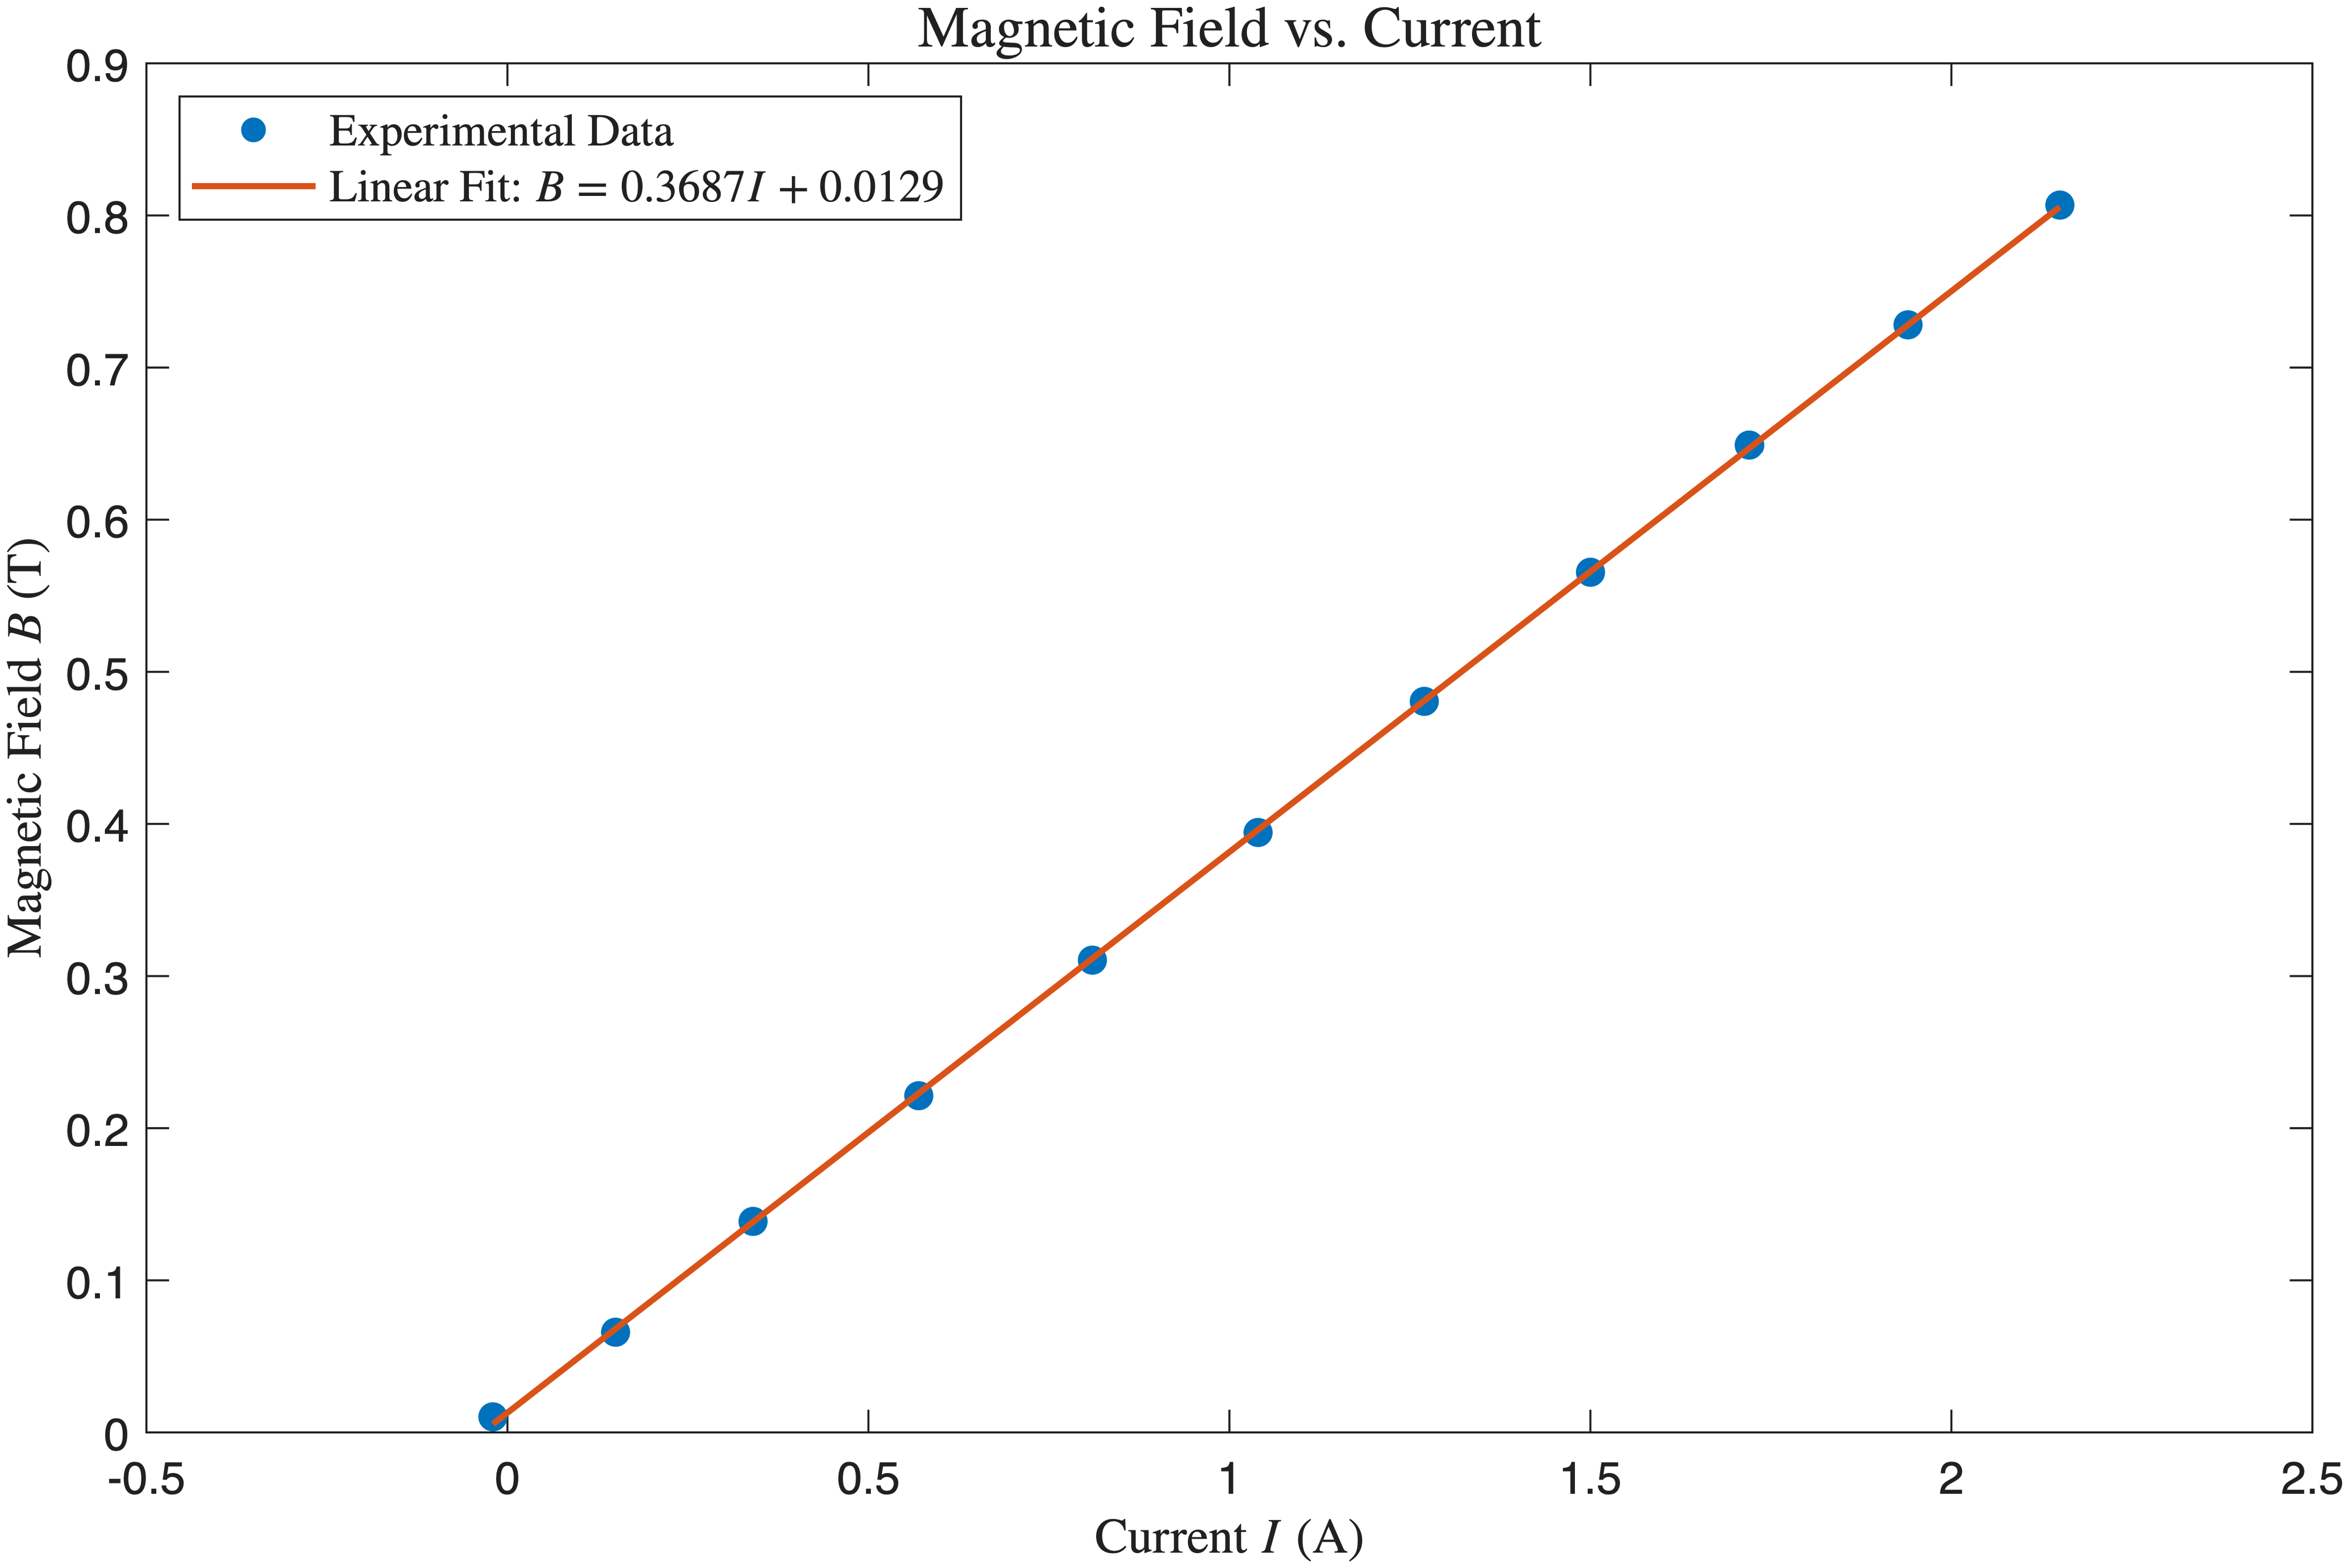
\includegraphics[width=\textwidth]{fig/IB.png}
    \caption{磁场定标曲线}
    \label{fig:IB}
\end{figure}

由实验数据可见，磁感应强度与电流之间呈现良好的线性关系($R^2 = 0.9998$)。对数据进行线性拟合，得到
\begin{equation}
    B = 0.3687 I + 0.0129
\end{equation}

其中 $B$ 的单位为 T，$I$ 的单位为 A。

\vspace{0.5em}

\textbf{旋光方向判据说明：}

记实验中光源位置为A，磁光调制器位置为B，则光传播方向为由A到B，定标实验中测得磁场方向为从B到A。一般约定，旋转方向与产生磁场的螺线管中电流方向一致时，法拉第旋转是左旋的，即$V(\lambda)>0$；反之则$V(\lambda)<0$，法拉第旋转是右旋的。


\subsubsection{磁场均匀性考察}

在固定电流 $I=1.8$ A 条件下，测量不同位置磁场强度。实验结果表明磁场在中心区域较为均匀，可近似认为样品处磁场均匀。


\subsection{旋光角测量}

\subsubsection{无样品无磁场的消光角度测量}
首先在无样品、无磁场条件下测量消光角，得到
\begin{equation}
    \alpha_0 = 52^\circ
\end{equation}
该角度为后续测量中旋光角的基准点，所有测量的旋光角均以此为参考进行计算。

\subsubsection{MR3-2 样品旋光角测量}

将 MR3-2 样品置于磁隙中，调节光路并利用倍频法确定无磁场消光角：
\begin{equation}
    \alpha_0^{\text{MR3}} = 51^\circ 34'
\end{equation}

在不同磁场条件下，分别采用倍频法与消光法测量旋光角变化。将两种方法得到的数据统一绘制在同一 $\theta-B$ 图中，以便进行直接比较：

\begin{figure}[h!]
    \centering
    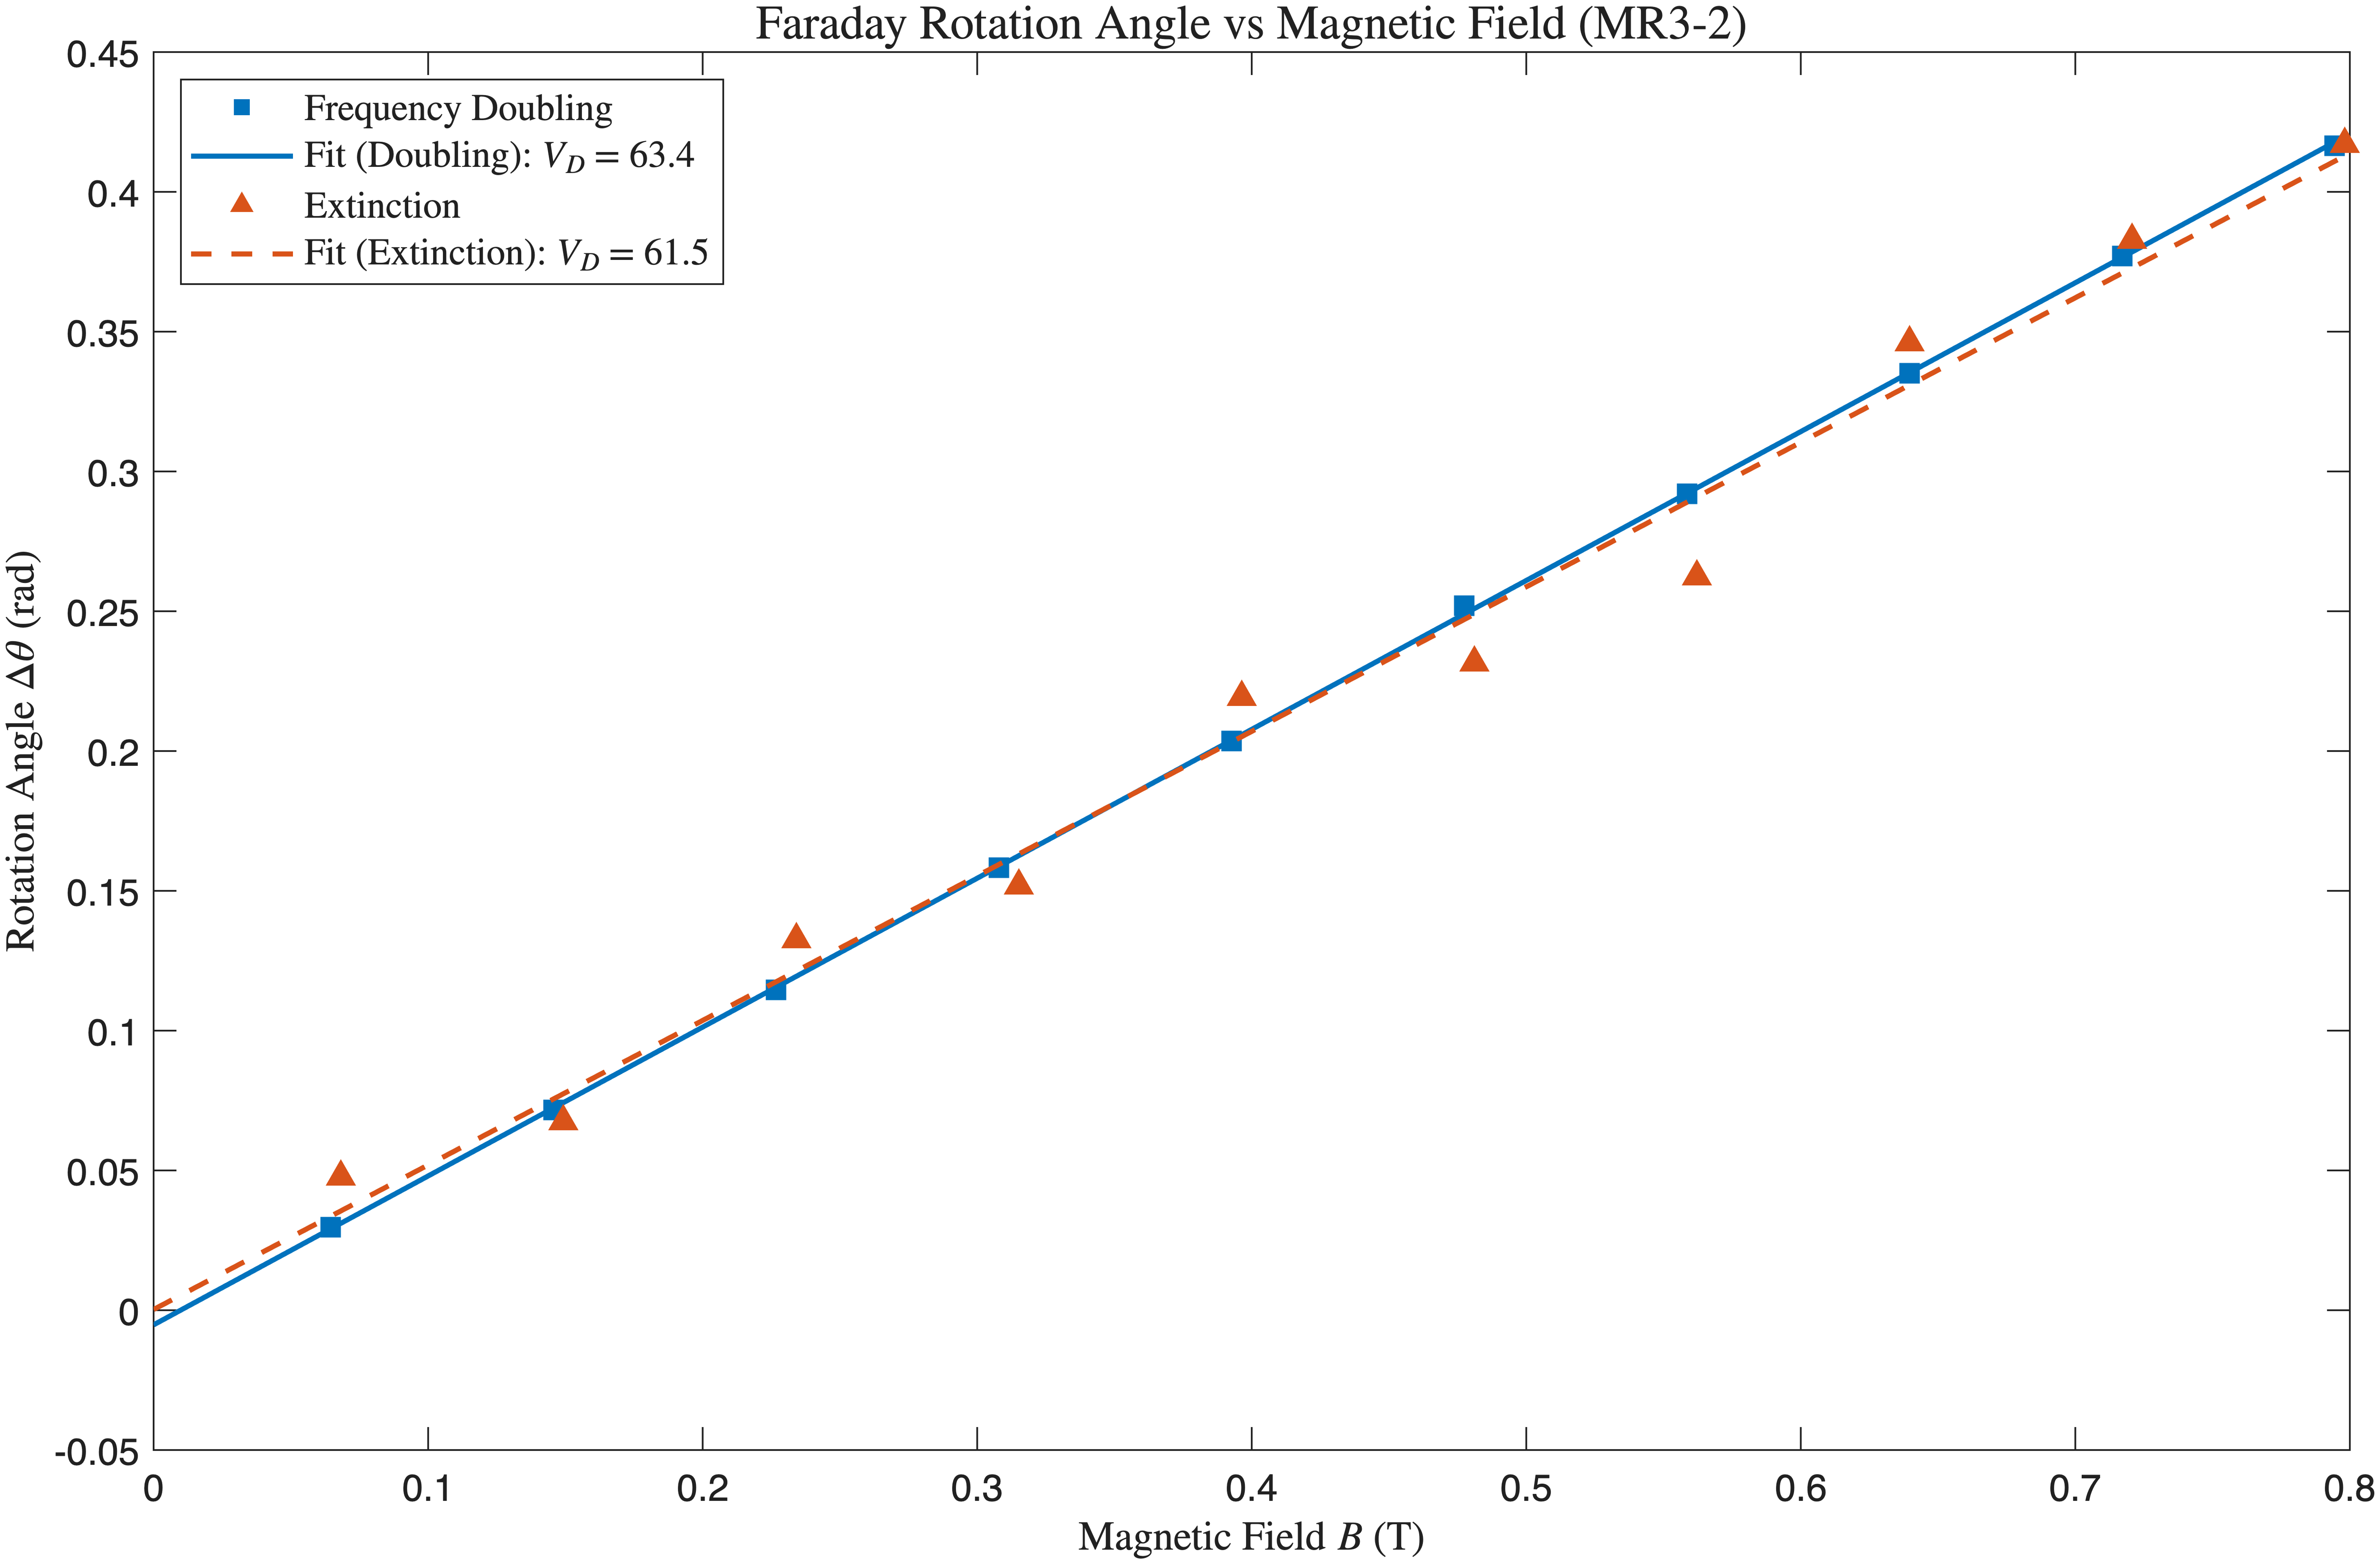
\includegraphics[width=\textwidth]{fig/mr32_b.png}
    \caption{MR3-2 样品 $\theta-B$ 曲线（倍频法与消光法对比）}
\end{figure}

可以看出，两种方法得到的数据整体一致，均呈现良好的线性关系，仅在个别点存在一定偏差。这说明倍频法与消光法在本实验条件下具有较好的一致性。

对倍频法数据进行线性拟合，得到：
\begin{equation}
    \dfrac{\mathrm{d}\theta}{\mathrm{d}B} = 0.5325 \, \mathrm{T}^{-1}
\end{equation}

可判断该样品为左旋光，其费尔德常数为
\begin{equation}
    V_d = 63.38 \, \mathrm{T}^{-1} \cdot \mathrm{m}^{-1}
\end{equation}

对消光法数据进行线性拟合，得到：
\begin{equation}
    \dfrac{\mathrm{d}\theta}{\mathrm{d}B} = 0.5169 \, \mathrm{T}^{-1}
\end{equation}

其费尔德常数为
\begin{equation}
    V_d = 61.54\, \mathrm{T}^{-1} \cdot \mathrm{m}^{-1}
\end{equation}


同时可以看出，自然旋光角较小，对总旋光贡献影响有限。


\subsubsection{ZF7 样品旋光角测量}

更换为 ZF7 样品后，重新调节光路并测得无磁场消光角：
\begin{equation}
    \alpha_0^{\text{ZF7}} = 52^\circ 20'
\end{equation}

在测量过程中分别记录电流上升和下降过程中的数据，并将两组数据绘制在同一图中：

\begin{figure}[h!]
    \centering
    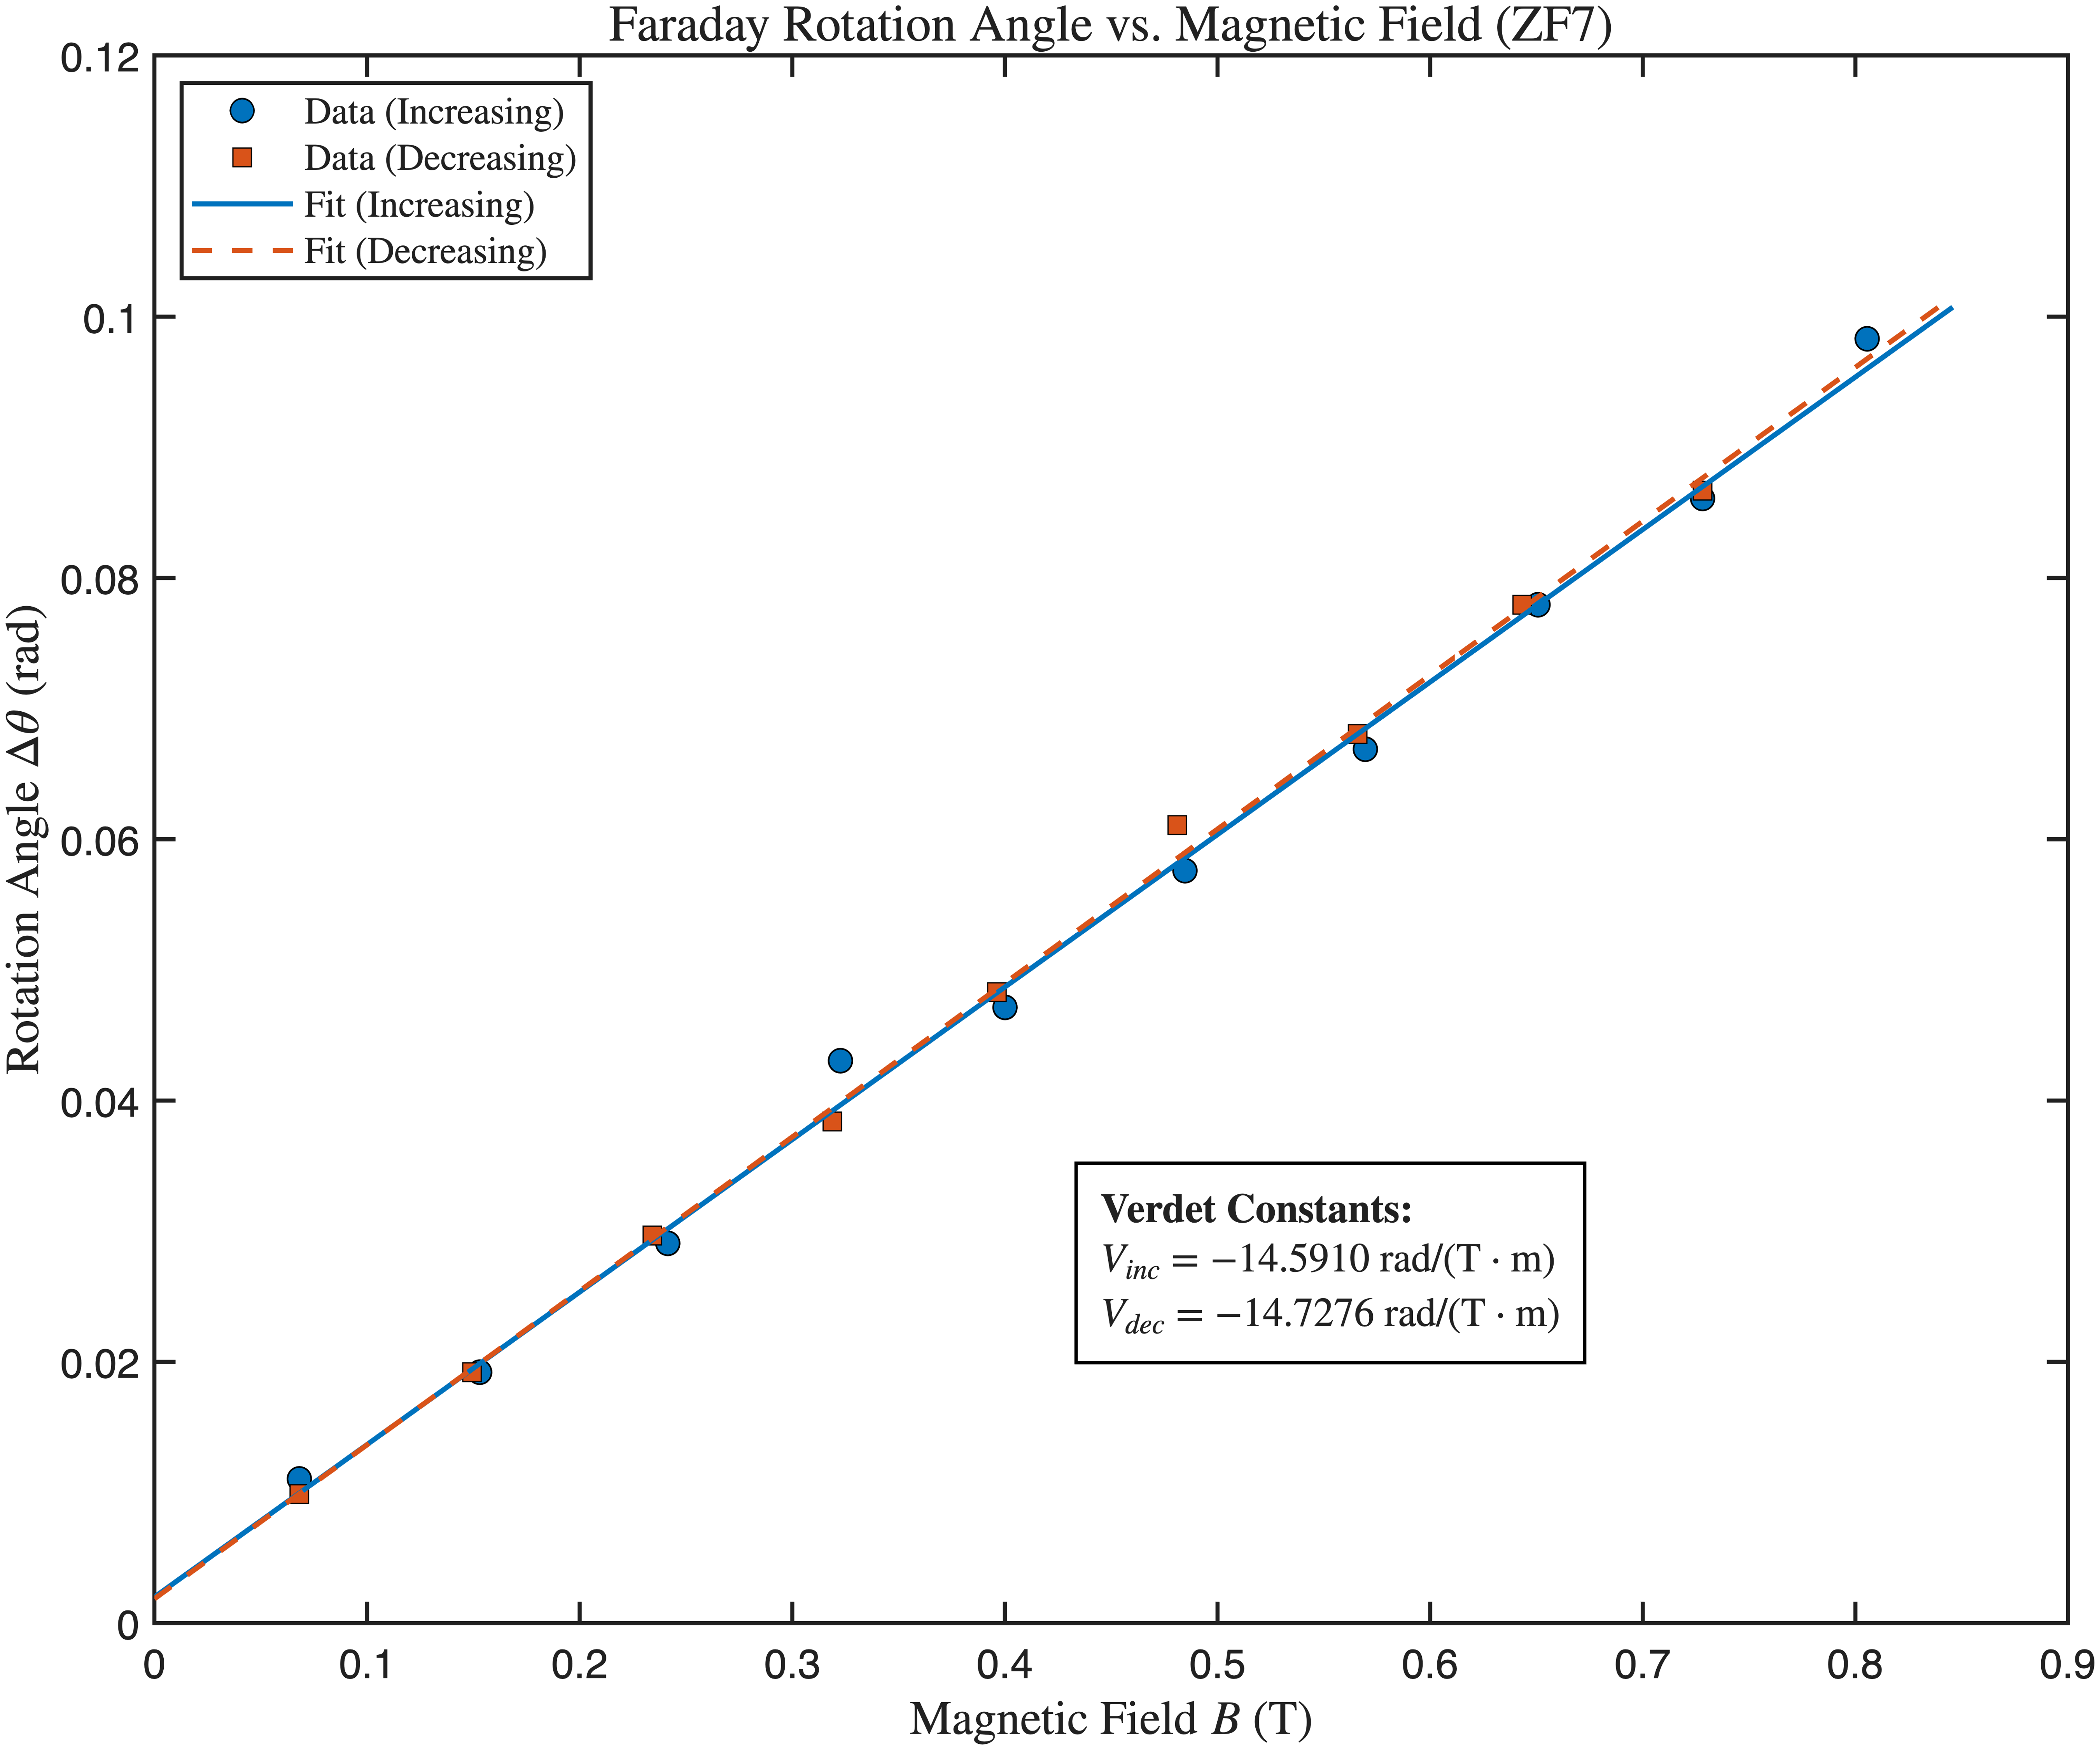
\includegraphics[width=\textwidth]{fig/zf7.png}
    \caption{ZF7 样品 $\theta-B$ 曲线（上升与下降过程对比）}
\end{figure}

实验结果显示，上升与下降过程的数据整体趋势一致，但可能存在轻微偏移，这反映了系统中可能存在的滞后效应或测量误差。

对数据进行线性拟合，且可判断该样品为右旋光，其费尔德常数为
\begin{equation}
    V_d = -14.59 \, \mathrm{T}^{-1} \cdot \mathrm{m}^{-1}
\end{equation}

该样品的自然旋光角较小，其影响在实验误差范围内。


\subsubsection{石英样品旋光角测量}

最后对石英样品进行测量，利用倍频法得到无磁场消光角：
\begin{equation}
    \alpha_0^{\text{Quartz}} = 306^\circ 48'
\end{equation}

在不同磁场条件下测量旋光角变化，得到 $\theta-B$ 曲线：

\begin{figure}[h!]
    \centering
    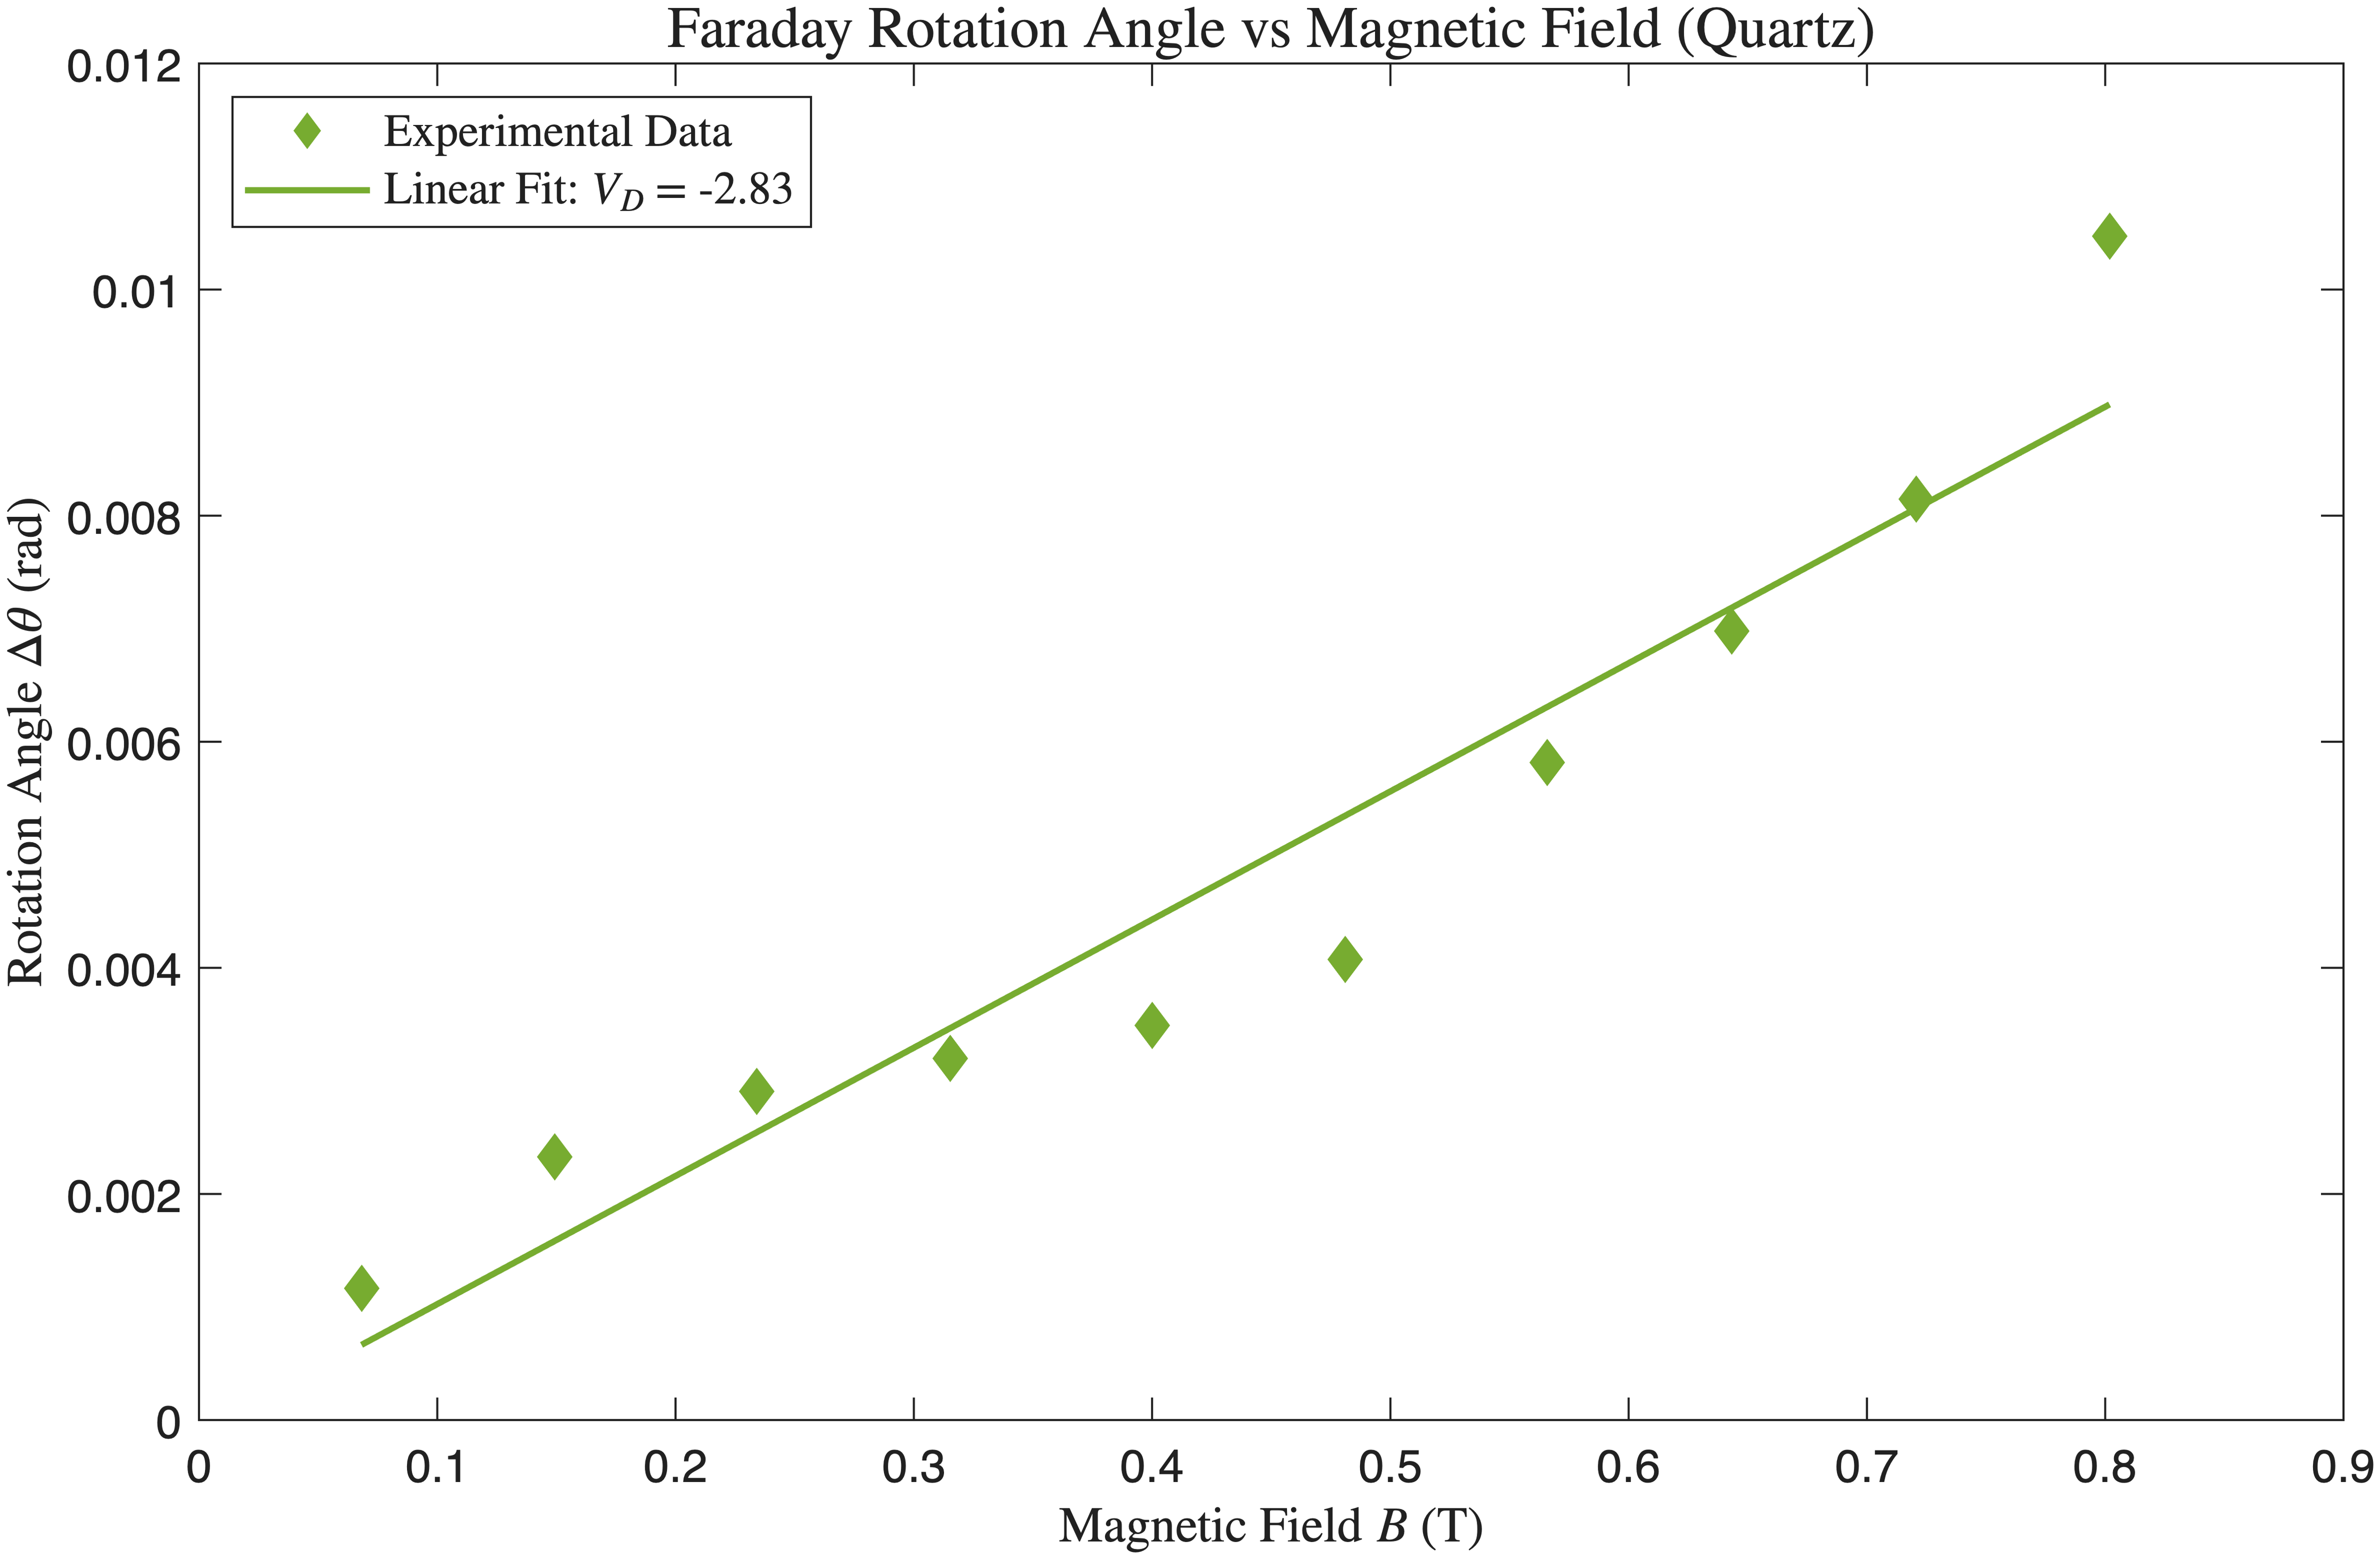
\includegraphics[width=\textwidth]{fig/quartz.png}
    \caption{石英样品 $\theta-B$ 曲线}
\end{figure}

对数据进行线性拟合，且可判断该样品为右旋光，其费尔德常数为
\begin{equation}
    V_d = -2.8349 \, \mathrm{T}^{-1} \cdot \mathrm{m}^{-1}
\end{equation}

可以看出，石英样品的磁致旋光效应较弱，而自然旋光贡献较为显著，因此测量结果更容易受到角度读数误差的影响。
\subsection{磁致旋光非互易性的验证}

为验证法拉第效应的非互易性，本实验通过改变光路，使光在样品中往返传播，并分别测量石英与 MR3-2 样品在有无磁场条件下的旋光角变化。

\subsubsection{石英样品的测量结果}

首先对石英样品进行测量。在无磁场条件下记录消光角为
\begin{equation*}
    \theta_0^{\text{(石英)}} = 231^\circ 2'
\end{equation*}

在加入磁场后，测得不同电流下的旋光角变化如下：
\begin{table}[h!]
    \centering
    \begin{tabular}{cc}
        \toprule
        电流 $I$/A & 旋光角 $\theta$ \\
        \midrule
        $0.99$ & $230^\circ 28'$ \\
        $1.86$ & $229^\circ 4'$ \\
        \bottomrule
    \end{tabular}
    \caption{石英样品磁致旋光测量数据}
\end{table}

可以看到，在磁场存在时，旋光角发生变化，但整体变化较小。这是由于石英的费尔德常数较小，其磁致旋光效应较弱。同时，由于光在样品中往返传播，自然旋光部分在正反路径中相互抵消，因此测得的变化主要来源于磁致旋光。

\subsubsection{MR3-2 样品的测量结果}

随后对 MR3-2 样品进行测量。首先记录近似无磁场条件下的消光角作为基准：
\begin{equation*}
    \theta_0^{\text{(MR3-2)}} = 228^\circ 06'
\end{equation*}

在加入磁场后，测得旋光角随电流变化如下：
\begin{table}[h!]
    \centering
    \begin{tabular}{cc}
        \toprule
        电流 $I$/A & 旋光角 $\theta$ \\
        \midrule
        $0.57$ & $236^\circ 18'$ \\
        $1.03$ & $251^\circ 48'$ \\
        $1.49$ & $261^\circ 30'$ \\
        $1.82$ & $272^\circ 22'$ \\
        \bottomrule
    \end{tabular}
    \caption{MR3-2 样品磁致旋光测量数据}
\end{table}

可以明显观察到，随着电流（磁场强度）增加，旋光角单调增大，且变化幅度远大于石英样品。这表明 MR3-2 具有显著的磁致旋光效应。

\subsubsection{非互易性的验证与分析}

实验结果表明：

在光往返通过样品的过程中，
\begin{itemize}
    \item 自然旋光：在正反传播过程中旋转方向相反，因此相互抵消；
    \item 磁致旋光：旋转方向仅由磁场方向决定，与传播方向无关，因此两次旋转发生叠加。
\end{itemize}

对于石英样品，由于其费尔德常数较小，磁致旋光效应较弱，因此往返传播后的旋光角变化不显著。

而对于 MR3-2 样品，由于其费尔德常数较大，磁致旋光效应明显，在往返传播过程中旋光角显著增加，验证了法拉第效应的\textbf{非互易性}。

此外，从 MR3-2 的测量数据可以看出，旋光角随电流近似呈线性增长趋势，这与理论关系
\begin{equation}
    \theta_F = V_d B l
\end{equation}
一致。

需要指出的是，实验中旋光角的增量可能略偏离理想的两倍关系，其原因可能包括光束未完全沿磁场方向传播、样品存在微小倾角导致有效光程增加，以及磁场分布不均匀等因素。

\section{总结}

本实验围绕法拉第效应的基本规律，对磁场与旋光角之间的关系进行了系统测量，并对不同材料的磁致旋光性质进行了对比分析。

首先，通过对电磁铁的 $I-B$ 关系进行标定，验证了磁感应强度与电流之间具有良好的线性关系，从而为后续旋光角与磁场的定量分析提供了可靠基础。同时，磁场在样品区域内具有较好的均匀性，使得实验中可以将磁场近似视为均匀分布。

在旋光角测量部分，三种样品均表现出旋光角随磁场变化近似线性的特征，符合 $\theta_F = V_d B l$ 的理论预期。其中：

MR3-2 样品表现出最显著的磁致旋光效应，其旋光角随磁场变化幅度较大，且倍频法与消光法测量结果具有良好一致性，说明两种方法在本实验条件下均具有较高可靠性；

ZF7 样品的磁致旋光效应明显弱于 MR3-2，但仍可清晰分辨，其测量结果在电流上升与下降过程中基本一致，仅存在轻微滞后现象，反映了系统中的非理想因素；

石英样品的磁致旋光效应最弱，其旋光角变化幅度较小，自然旋光贡献相对占主导，使得测量结果更易受到读数误差影响。

进一步地，通过构造光在样品中往返传播的实验路径，对法拉第效应的非互易性进行了验证。实验结果表明，自然旋光在往返过程中相互抵消，而磁致旋光则发生叠加。该效应在 MR3-2 样品中表现尤为明显，而在石英样品中则由于费尔德常数较小而不显著。这一结果从实验上直接体现了磁致旋光“与传播方向无关”的本质特征。

总体而言，本实验不仅验证了法拉第效应的基本线性规律，还通过不同材料的对比分析揭示了费尔德常数对磁致旋光强度的决定性作用，并通过非互易性实验深化了对磁光效应物理本质的理解。
    \begin{thebibliography}{99}
        \bibitem{1}
        北京师范大学物理实验教学中心. 近代物理实验讲义一 (2019)
    \end{thebibliography}

\end{document}